\documentclass[aspectratio=169,11pt,t]{beamer}

% ============================================================
% Theme and typography
% ============================================================

\usetheme{Madrid}
\usecolortheme{default}
\usefonttheme{professionalfonts}

\setbeamertemplate{navigation symbols}{}
\setbeamertemplate{headline}{}

\setbeamertemplate{footline}{%
  \leavevmode\hbox{%
  \begin{beamercolorbox}[wd=.82\paperwidth,ht=2.5ex,dp=1.0ex,leftskip=.8em]{author in head/foot}
    CSCI 6461 --- Computer Systems Architecture
  \end{beamercolorbox}%
  \begin{beamercolorbox}[wd=.18\paperwidth,ht=2.5ex,dp=1.0ex,rightskip=.8em]{date in head/foot}
    \hfill\insertframenumber/\inserttotalframenumber
  \end{beamercolorbox}}
}

\setbeamersize{text margin left=0.7cm,text margin right=0.7cm}
\setbeamerfont{frametitle}{size=\Large,series=\bfseries}
\setbeamerfont{block title}{size=\normalsize,series=\bfseries}
\setbeamertemplate{blocks}[rounded][shadow=false]
\setbeamertemplate{itemize/enumerate body begin}{\setlength{\itemsep}{4pt}}
\setbeamertemplate{itemize/enumerate subbody begin}{\setlength{\itemsep}{2pt}}

\usepackage[T1]{fontenc}
\usepackage{lmodern}
\usepackage{amsmath}
\usepackage{booktabs}
\usepackage{array}
\usepackage{tikz}
\usetikzlibrary{
  arrows.meta,
  positioning,
  shapes.geometric,
  calc,
  decorations.pathreplacing
}

\definecolor{navy}{RGB}{24,43,68}
\definecolor{deepblue}{RGB}{45,88,130}
\definecolor{lightblue}{RGB}{235,242,250}
\definecolor{softgray}{RGB}{245,247,250}
\definecolor{darkgray}{RGB}{25,28,32}
\definecolor{gold}{RGB}{200,145,35}

\setbeamercolor{palette primary}{bg=navy,fg=white}
\setbeamercolor{palette secondary}{bg=deepblue,fg=white}
\setbeamercolor{frametitle}{bg=navy,fg=white}
\setbeamercolor{title}{fg=white}
\setbeamercolor{subtitle}{fg=white}
\setbeamercolor{author}{fg=white}
\setbeamercolor{date}{fg=white}
\setbeamercolor{titlelike}{fg=white}
\setbeamercolor{block title}{bg=deepblue,fg=white}
\setbeamercolor{block body}{bg=lightblue,fg=darkgray}
\setbeamercolor{normal text}{fg=darkgray,bg=white}

\setlength{\parskip}{0pt}

\newcommand{\key}[1]{\textbf{#1}}
\newcommand{\bits}[1]{\texttt{#1}}
\newcommand{\hex}[1]{\texttt{0x#1}}
\newcommand{\code}[1]{\texttt{#1}}

\newcommand{\sectiondivider}[2]{%
\begin{frame}[plain]
\begin{tikzpicture}[remember picture,overlay]
\fill[navy] (current page.south west) rectangle (current page.north east);
\fill[gold] (current page.south west) rectangle ([yshift=.15cm]current page.south east);
\end{tikzpicture}
\vspace{1.5cm}
\begin{minipage}{0.85\textwidth}
{\color{gold}\large\bfseries #1\par}
\vspace{0.3cm}
{\color{white}\fontsize{22}{26}\selectfont\bfseries #2\par}
\end{minipage}
\end{frame}
}

\title[Topic 1]{Introduction to Computing Systems\\\& Binary Foundations}
\subtitle{Abstraction, stored-program organization, data representation, and processor performance}
\author{Computer Systems Architecture}
\date{}

\begin{document}

% ============================================================
% Slide 1
% ============================================================

% Slide 1
\begin{frame}[plain]
\begin{tikzpicture}[remember picture,overlay]
\fill[navy] (current page.south west) rectangle (current page.north east);
\fill[gold] (current page.south west) rectangle ([yshift=.15cm]current page.south east);
\end{tikzpicture}

\vspace{0.9cm}

\begin{minipage}{0.88\textwidth}
{\color{gold}\normalsize\bfseries CSCI 6461 \;|\; TOPIC 1\par}

\vspace{0.25cm}

{\color{white}\fontsize{24}{28}\selectfont\bfseries
Introduction to Computing Systems\\[0.08cm]
\& Binary Foundations
\par}

\vspace{0.35cm}

{\color{white!80}\large
Abstraction, stored-program organization, data representation, and processor performance
\par}
\end{minipage}

\vfill

{\color{white}\normalsize Dr. J. Burns\par}
{\color{white!70}\small Computer Systems Architecture --- AArch64 Reference Platform\par}

\vspace{0.35cm}
\end{frame}

% ============================================================
% PART 1
% ============================================================

\sectiondivider{PART 1}{Architecture Foundations \& Abstraction}

% ============================================================
% Slide 2
% ============================================================

% Slide 2
\begin{frame}{What Is Computer Architecture?}

\begin{itemize}\setlength{\itemsep}{7pt}
  \item Computer architecture connects \key{software-visible behavior} with \key{hardware implementation}.
  \item Hardware provides an interface that software can rely on.
  \item The implementation of that interface determines performance and efficiency.
  \item Architectural design involves correctness, performance, power, area, and cost.
\end{itemize}

\vspace{0.35cm}

\begin{block}{Course Approach}
\key{Design approach:} RISC principles.\\
\key{Reference ISA:} AArch64.
\end{block}

\end{frame}

% ============================================================
% Slide 3: The Full Abstraction Stack
% ============================================================

% Slide 3
\begin{frame}{The 9 Levels of Computer Abstraction}
    Computers manage immense complexity by enforcing clean hierarchical interfaces:
    \vspace{0.2em}
    \begin{center}
        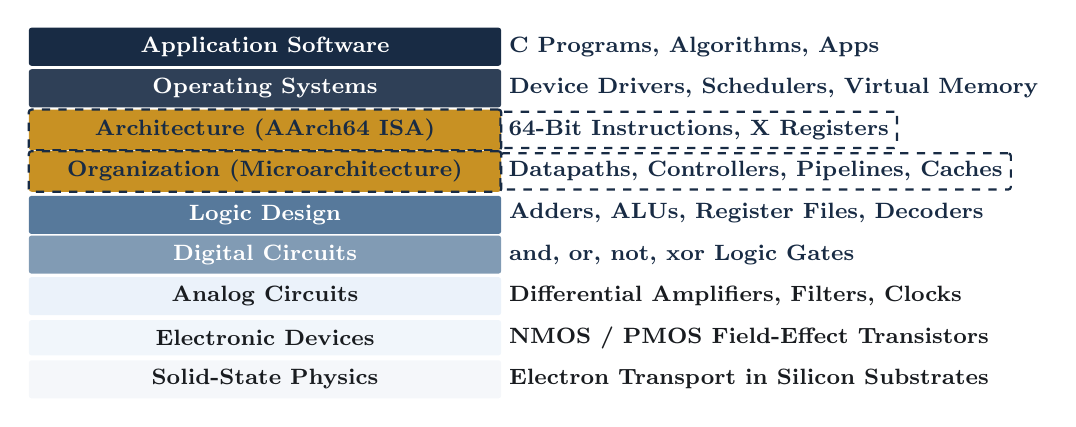
\begin{tikzpicture}[xscale=0.85, yscale=0.48, every node/.style={font=\footnotesize\bfseries}]
            \node[fill=navy, text=white, minimum width=6cm, minimum height=0.45cm, rounded corners=1pt] at (0,8.2) {Application Software};
            \node[fill=navy!90, text=white, minimum width=6cm, minimum height=0.45cm, rounded corners=1pt] at (0,7.1) {Operating Systems};
            \node[fill=gold, text=navy, minimum width=6cm, minimum height=0.45cm, rounded corners=1pt, draw=navy, thick, dashed] at (0,6.0) {Architecture (AArch64 ISA)};
            \node[fill=gold, text=navy, minimum width=6cm, minimum height=0.45cm, rounded corners=1pt, draw=navy, thick, dashed] at (0,4.9) {Organization (Microarchitecture)};
            \node[fill=deepblue!80, text=white, minimum width=6cm, minimum height=0.45cm, rounded corners=1pt] at (0,3.75) {Logic Design};
            \node[fill=deepblue!60, text=white, minimum width=6cm, minimum height=0.45cm, rounded corners=1pt] at (0,2.7) {Digital Circuits};
            \node[fill=lightblue, text=darkgray, minimum width=6cm, minimum height=0.45cm, rounded corners=1pt] at (0,1.6) {Analog Circuits};
            \node[fill=lightblue!70, text=darkgray, minimum width=6cm, minimum height=0.45cm, rounded corners=1pt] at (0,0.5) {Electronic Devices};
            \node[fill=softgray, text=darkgray, minimum width=6cm, minimum height=0.45cm, rounded corners=1pt] at (0,-0.6) {Solid-State Physics};

            \node[anchor=west, text=navy] at (3.5,8.2) {C Programs, Algorithms, Apps};
            \node[anchor=west, text=navy] at (3.5,7.1) {Device Drivers, Schedulers, Virtual Memory};
            \node[anchor=west, text=navy, draw=navy, thick, dashed, inner sep=3pt, rounded corners=1pt] at (3.5,6.0) {\textbf{64-Bit Instructions, X Registers}};
            \node[anchor=west, text=navy, draw=navy, thick, dashed, inner sep=3pt, rounded corners=1pt] at (3.5,4.9) {\textbf{Datapaths, Controllers, Pipelines, Caches}};
            \node[anchor=west, text=navy] at (3.5,3.8) {Adders, ALUs, Register Files, Decoders};
            \node[anchor=west, text=navy] at (3.5,2.7) {and, or, not, xor Logic Gates};
            \node[anchor=west, text=darkgray] at (3.5,1.6) {Differential Amplifiers, Filters, Clocks};
            \node[anchor=west, text=darkgray] at (3.5,0.5) {NMOS / PMOS Field-Effect Transistors};
            \node[anchor=west, text=darkgray] at (3.5,-0.6) {Electron Transport in Silicon Substrates};
        \end{tikzpicture}
    \end{center}
\end{frame}

% ============================================================
% Slide 4
% ============================================================

% Slide 4
\begin{frame}{When Abstractions Leak}

\begin{columns}[T,onlytextwidth]
\column{0.48\textwidth}
\begin{block}{Software View}
\begin{itemize}
  \item Variables, Arrays, Branches
  \item Function calls, Data types
\end{itemize}
\end{block}

\column{0.48\textwidth}
\begin{block}{Architectural Effect}
\begin{itemize}
  \item Register allocation, Cache misses
  \item Branch prediction, Stack frames
  \item Overflow and sign extension
\end{itemize}
\end{block}
\end{columns}

\vspace{0.35cm}
Performance-sensitive software often exposes lower-level machine behavior.
\end{frame}

% ============================================================
% Slide 5
% ============================================================

% Slide 5
\begin{frame}{From Source Code to Execution}

\centering
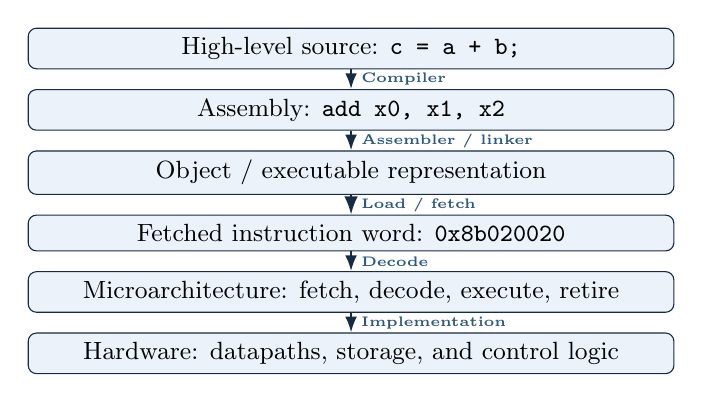
\begin{tikzpicture}[
  node distance=0.25cm,
  box/.style={
    rounded corners=3pt,
    draw=navy,
    fill=lightblue,
    align=center,
    font=\small,
    minimum width=8.2cm,
    minimum height=0.42cm
  }
]
\node[box] (c) {High-level source: \code{c = a + b;}};
\node[box, below=of c] (asm) {Assembly: \code{add x0, x1, x2}};
\node[box, below=of asm] (obj) {Object / executable representation};
\node[box, below=of obj] (inst) {Fetched instruction word: \code{0x8b020020}};
\node[box, below=of inst] (uarch) {Microarchitecture: fetch, decode, execute, retire};
\node[box, below=of uarch] (logic) {Hardware: datapaths, storage, and control logic};

\draw[-{Latex[length=2mm]}, thick, navy] (c) -- (asm) node[midway,right,font=\tiny\bfseries,text=deepblue]{Compiler};
\draw[-{Latex[length=2mm]}, thick, navy] (asm) -- (obj) node[midway,right,font=\tiny\bfseries,text=deepblue]{Assembler / linker};
\draw[-{Latex},thick, navy] (obj) -- (inst) node[midway,right,font=\tiny\bfseries,text=deepblue]{Load / fetch};
\draw[-{Latex[length=2mm]}, thick, navy] (inst) -- (uarch) node[midway,right,font=\tiny\bfseries,text=deepblue]{Decode};
\draw[-{Latex[length=2mm]}, thick, navy] (uarch) -- (logic) node[midway,right,font=\tiny\bfseries,text=deepblue]{Implementation};
\end{tikzpicture}

\vspace{0.15cm}
\small
The ISA is the boundary between program representation and processor execution.
\end{frame}

% ============================================================
% Slide 6
% ============================================================

% Slide 6
\begin{frame}{ISA and Microarchitecture}

\begin{columns}[T,onlytextwidth]
\column{0.48\textwidth}
\begin{block}{Instruction Set Architecture}
\begin{itemize}
  \item Instruction encodings \& behavior
  \item Registers \bits{x0}--\bits{x30}, \bits{sp}, PSTATE
  \item Memory and exception behavior
\end{itemize}
\end{block}

\column{0.48\textwidth}
\begin{block}{Microarchitecture}
\begin{itemize}
  \item Pipeline organization, Superscalar width
  \item In-order or out-of-order execution
  \item Branch prediction, Cache structures
\end{itemize}
\end{block}
\end{columns}

\vspace{0.25cm}
Different processors can implement the same ISA using different microarchitectures.
\end{frame}

% ============================================================
% Slide 7
% ============================================================

% Slide 7
\begin{frame}{RISC Design Principles and AArch64 Encoding}

\begin{itemize}\setlength{\itemsep}{5pt}
  \item RISC designs emphasize regular instruction formats and explicit load/store architecture.
  \item AArch64 instructions are fixed-width \key{32-bit words}, aligned on 4-byte boundaries.
  \item Destination (\code{Rd}) and source operands (\code{Rn}, \code{Rm}) use fixed 5-bit register fields ($2^5 = 32$).
\end{itemize}

\vspace{0.15cm}
\begin{block}{Example: 64-Bit Addition (\texttt{add x0, x1, x2} $\implies$ \texttt{0x8b020020})}
\centering
\small Encoding maps \code{Rd = x0}, \code{Rn = x1}, \code{Rm = x2} within the uniform 32-bit word.
\end{block}

\end{frame}

% ============================================================
% PART 2
% ============================================================

\sectiondivider{PART 2}{Stored-Program Organization \& Memory}

% ============================================================
% Slide 8
% ============================================================

% Slide 8
\begin{frame}{The Stored-Program Concept \& Execution Cycle}

\begin{itemize}\setlength{\itemsep}{5pt}
  \item Instructions and data share a unified memory space, encoded as binary numbers.
  \item The processor maintains a Program Counter (\bits{pc}) pointing to the next instruction.
\end{itemize}

\vspace{0.15cm}
\centering
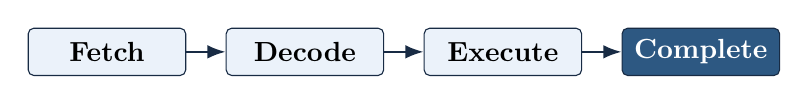
\begin{tikzpicture}[node distance=0.5cm]
\node[draw=navy, fill=lightblue, rounded corners=2pt, minimum width=2.0cm, minimum height=0.6cm, font=\bfseries] (f) {Fetch};
\node[draw=navy, fill=lightblue, rounded corners=2pt, right=of f, minimum width=2.0cm, minimum height=0.6cm, font=\bfseries] (d) {Decode};
\node[draw=navy, fill=lightblue, rounded corners=2pt, right=of d, minimum width=2.0cm, minimum height=0.6cm, font=\bfseries] (e) {Execute};
\node[draw=navy, fill=deepblue, text=white, rounded corners=2pt, right=of e, minimum width=2.0cm, minimum height=0.6cm, font=\bfseries] (w) {Complete};

\draw[-{Latex},thick,navy] (f)--(d);
\draw[-{Latex},thick,navy] (d)--(e);
\draw[-{Latex},thick,navy] (e)--(w);
\end{tikzpicture}

\vspace{0.2cm}
Real processors overlap instruction execution via pipelining, while branches and exceptions alter the standard sequential flow.
\end{frame}

% ============================================================
% Slide 9
% ============================================================

% Slide 9
\begin{frame}{Memory Topologies: von Neumann, Harvard, Modified Harvard}

\begin{columns}[T,onlytextwidth]
\column{0.32\textwidth}
\begin{block}{von Neumann}
Shared memory and bus path; instruction and data access contend for bandwidth.
\end{block}

\column{0.32\textwidth}
\begin{block}{Pure Harvard}
Separate memories and buses for code and data; enables parallel access.
\end{block}

\column{0.32\textwidth}
\begin{block}{Modified Harvard}
Unified software address space with split L1 instruction and data caches.
\end{block}
\end{columns}

\vspace{0.25cm}
Modern high-performance processors (including AArch64) utilize Modified Harvard topologies.
\end{frame}

% ============================================================
% Slide 10
% ============================================================

% Slide 10
\begin{frame}{Modified Harvard \& Self-Modifying Code (SMC)}

\begin{itemize}\setlength{\itemsep}{5pt}
  \item Split L1 $I\text{-cache}$ and $D\text{-cache}$ require explicit synchronization when runtime compilers (JIT) write code as data.
  \item AArch64 requires explicit cache cleaning, barrier instructions, and instruction invalidation:
\end{itemize}

\vspace{0.15cm}
\begin{block}{Required Synchronization Sequence}
\small
\code{dc cvau, x0} $\to$ \code{dsb ish} $\to$ \code{ic ivau, x0} $\to$ \code{dsb ish} $\to$ \code{isb}
\end{block}

\vspace{0.15cm}
Ensures visibility between data modifications and subsequent instruction fetches.
\end{frame}

% ============================================================
% Slide 11
% ============================================================

% Slide 11
\begin{frame}{Memory Hierarchy \& The Memory Wall}

\begin{columns}[T,onlytextwidth]
\column{0.50\textwidth}
\begin{block}{Hierarchy Tiers}
\begin{itemize}\setlength{\itemsep}{2pt}
  \item \key{Registers:} $\approx 1$ cycle
  \item \key{L1 Cache:} $3\text{--}4$ cycles
  \item \key{L2/L3 Cache:} $10\text{--}60$ cycles
  \item \key{DRAM (Main Memory):} $200\text{+}$ cycles
  \item \key{Persistent Storage:} SSD/NVMe
\end{itemize}
\end{block}

\column{0.46\textwidth}
\begin{block}{The Memory Wall}
Processor compute capability scales much faster than DRAM latency, making cache management, locality, and prefetching critical to performance.
\end{block}
\end{columns}

\end{frame}

% ============================================================
% PART 3
% ============================================================

\sectiondivider{PART 3}{Binary Representation \& Arithmetic}

% ============================================================
% Slide 12
% ============================================================

% Slide 12
\begin{frame}{Bits and Interpretive Context}

\begin{itemize}\setlength{\itemsep}{5pt}
  \item Hardware stores uninterpreted binary bit patterns ($\{0, 1\}^n$).
  \item An $n$-bit field yields $2^n$ combinations; meaning depends entirely on the active instruction context.
\end{itemize}

\vspace{0.15cm}
\begin{center}
\footnotesize
\begin{tabular}{ll}
\toprule
\textbf{Interpretation Perspective} & \textbf{Meaning of 32-bit Word \hex{8b020020}} \\
\midrule
AArch64 Machine Instruction & \code{add x0, x1, x2} \\
Unsigned 32-bit Integer     & $2{,}332{,}164{,}128_{10}$ \\
Signed 32-bit Integer       & $-1{,}962{,}803{,}168_{10}$ \\
\bottomrule
\end{tabular}
\end{center}

\end{frame}

% ============================================================
% Slide 13
% ============================================================

% Slide 13
\begin{frame}{Positional Systems \& Endianness}

\begin{itemize}\setlength{\itemsep}{5pt}
  \item \key{Positional Binary:} $\text{Value} = \sum_{i=0}^{n-1} b_i 2^i$. Hexadecimal compresses nibbles ($4\text{ bits} = 1\text{ hex digit}$).
  \item \key{Byte Ordering (Endianness):} Dictates how multi-byte values map to memory addresses.
  \begin{itemize}\setlength{\itemsep}{2pt}
    \item \textbf{Little-Endian (AArch64 / x86):} Least Significant Byte (LSB) stored at the lowest address.
    \item \textbf{Big-Endian:} Most Significant Byte (MSB) stored at the lowest address.
  \end{itemize}
\end{itemize}

\end{frame}

% ============================================================
% Slide 14
% ============================================================

% Slide 14
\begin{frame}{Two's-Complement Representation \& Ranges}

\begin{itemize}\setlength{\itemsep}{5pt}
  \item Signed integers utilize two's complement, where the MSB carries a negative positional weight ($-2^{n-1}$).
  \item \key{Negation Property:} $-x = \sim x + 1$.
\end{itemize}

\vspace{0.15cm}
\begin{columns}[T,onlytextwidth]
\column{0.48\textwidth}
\begin{block}{Unsigned Ranges ($0$ to $2^n - 1$)}
\begin{itemize}\setlength{\itemsep}{1pt}
  \item 8-bit: $0$ to $255$
  \item 32-bit: $0$ to $4.29 \times 10^9$
  \item 64-bit: $0$ to $1.84 \times 10^{19}$
\end{itemize}
\end{block}

\column{0.48\textwidth}
\begin{block}{Two's Complement ($-2^{n-1}$ to $2^{n-1}-1$)}
\begin{itemize}\setlength{\itemsep}{1pt}
  \item 8-bit: $-128$ to $+127$
  \item 32-bit: $\pm 2.14 \times 10^9$
  \item 64-bit: $\pm 9.22 \times 10^{18}$
\end{itemize}
\end{block}
\end{columns}

\end{frame}

% ============================================================
% Slide 15
% ============================================================

% Slide 15
\begin{frame}{Unified Adder Datapath \& Extension Rules}

\begin{itemize}\setlength{\itemsep}{4pt}
  \item The identical hardware adder supports signed and unsigned addition; subtraction uses $A - B = A + (\sim B) + 1$.
  \item \key{Promotion Rules:}
  \begin{itemize}\setlength{\itemsep}{2pt}
    \item \textbf{Sign Extension (\code{ldrsb}):} Replicates the MSB across upper bits to preserve negative values.
    \item \textbf{Zero Extension (\code{ldrb}):} Pads upper bits with zeros to preserve unsigned magnitude.
  \end{itemize}
\end{itemize}

\vspace{0.15cm}
\begin{block}{Security Warning}
Zero-extending a signed negative integer converts $-1$ into a massive positive value, breaking array bounds checks.
\end{block}

\end{frame}

% ============================================================
% Slide 16
% ============================================================

% Slide 16
\begin{frame}{AArch64 NZCV Condition Flags}

Arithmetic instructions can update status flags in PSTATE:

\vspace{0.15cm}
\small
\begin{center}
\begin{tabular}{cll}
\toprule
Flag & Name & Evaluation Meaning \\
\midrule
N & Negative & Result MSB is 1 (negative signed value) \\
Z & Zero     & All result bits are zero \\
C & Carry    & Unsigned carry-out (add) or No-Borrow ($\ge$, sub) \\
V & Overflow & Signed arithmetic overflow range violation \\
\bottomrule
\end{tabular}
\end{center}

\vspace{0.15cm}
Explicit flag-setting instructions use the \code{s} suffix (\code{adds}, \code{subs}, or alias \code{cmp}).
\end{frame}

% ============================================================
% Slide 17
% ============================================================

% Slide 17
\begin{frame}{Signed vs.\ Unsigned Conditional Branching}

After a comparison (\code{cmp x0, x1}), conditional branches test specific flag combinations:

\vspace{0.15cm}
\small
\begin{center}
\begin{tabular}{llll}
\toprule
Branch & Context & Flag Condition & Meaning \\
\midrule
\code{b.eq} / \code{b.ne} & Universal & $Z=1$ / $Z=0$ & Equal / Not Equal \\
\code{b.lt} / \code{b.ge} & \textbf{Signed} & $N \neq V$ / $N = V$ & Less Than / Greater or Equal \\
\code{b.lo} / \code{b.hs} & \textbf{Unsigned} & $C=0$ / $C=1$ & Lower ($<$) / Higher or Equal ($\ge$) \\
\bottomrule
\end{tabular}
\end{center}

\vspace{0.2cm}
Choosing the correct mnemonic (\code{b.lo} for memory pointers vs.\ \code{b.lt} for signed integers) is vital for correctness.
\end{frame}

% ============================================================
% PART 4
% ============================================================

\sectiondivider{PART 4}{Quantitative Processor Performance}

% ============================================================
% Slide 18
% ============================================================

% Slide 18
\begin{frame}{Defining Performance and Execution Time}

\begin{itemize}\setlength{\itemsep}{5pt}
  \item For a fixed workload, performance is inversely proportional to execution time:
  $$\text{Performance} = \frac{1}{\text{Execution Time}}$$
  \item \key{CPU Execution Time ($T_{\text{CPU}}$):} Time spent executing instructions on behalf of the application process.
  \item Clock period and frequency are reciprocals: $T_{\text{clk}} = \frac{1}{f_{\text{clk}}}$.
\end{itemize}

\vspace{0.15cm}
\begin{block}{Latency vs.\ Throughput}
\textbf{Latency:} Time to complete one task.\\
\textbf{Throughput:} Tasks completed per unit time (e.g., IPC).
\end{block}

\end{frame}

% ============================================================
% Slide 19
% ============================================================

% Slide 19
\begin{frame}{Dynamic Instruction Count vs.\ CPI}

\begin{itemize}\setlength{\itemsep}{5pt}
  \item \key{Dynamic Instruction Count (IC):} The actual number of instructions executed at runtime (dependent on inputs and loops).
  \item \key{Cycles Per Instruction (CPI):} Average clock cycles required per instruction:
  $$\text{CPI} = \frac{\text{Total Clock Cycles}}{\text{Dynamic Instruction Count}} \qquad \text{IPC} = \frac{1}{\text{CPI}}$$
  \item Modern \key{superscalar cores} fetch and execute multiple instructions per cycle in parallel ($\text{CPI} < 1.0$, or $\text{IPC} > 1.0$).
\end{itemize}

\end{frame}

% ============================================================
% Slide 20
% ============================================================

% Slide 20
\begin{frame}{The Iron Law of Processor Performance}

\begin{block}{The Fundamental CPU Performance Equation}
$$T_{\text{CPU}} = \text{Instruction Count (IC)} \times \text{CPI} \times T_{\text{clk}} = \frac{\text{IC} \times \text{CPI}}{f_{\text{clk}}}$$
\end{block}

\vspace{0.15cm}
\begin{center}
\footnotesize
\begin{tabular}{lll}
\toprule
Component & Influenced By & Design Trade-off \\
\midrule
\textbf{IC}   & Algorithm, Compiler, ISA & CISC vs.\ RISC instruction density \\
\textbf{CPI}  & Pipeline, Memory hierarchy & Out-of-order complexity, Cache misses \\
\textbf{$T_{\text{clk}}$} & Pipeline depth, Circuit nodes & Higher frequency requires deeper pipelines \\
\bottomrule
\end{tabular}
\end{center}

\end{frame}

% ============================================================
% Slide 21
% ============================================================

% Slide 21
\begin{frame}{Iron Law: Comparative Evaluation Example}

\begin{columns}[T,onlytextwidth]
\column{0.48\textwidth}
\begin{block}{Machine A (Deep Pipeline)}
\begin{itemize}\setlength{\itemsep}{1pt}
  \item $\text{IC} = 1.0 \times 10^9$
  \item $\text{CPI} = 2.0$
  \item $f_{\text{clk}} = 4.0\text{ GHz}$
\end{itemize}
$$T_A = \frac{1.0 \times 10^9 \times 2.0}{4.0 \times 10^9} = \mathbf{0.50\text{ s}}$$
\end{block}

\column{0.48\textwidth}
\begin{block}{Machine B (Wide Out-of-Order)}
\begin{itemize}\setlength{\itemsep}{1pt}
  \item $\text{IC} = 1.2 \times 10^9$ (+20\% IC)
  \item $\text{CPI} = 0.8$ (High IPC)
  \item $f_{\text{clk}} = 2.5\text{ GHz}$
\end{itemize}
$$T_B = \frac{1.2 \times 10^9 \times 0.8}{2.5 \times 10^9} = \mathbf{0.384\text{ s}}$$
\end{block}
\end{columns}

\vspace{0.2cm}
$$\text{Speedup} = \frac{T_A}{T_B} = \frac{0.50}{0.384} \approx \mathbf{1.30\times\text{ faster for Machine B}}$$

\end{frame}

% ============================================================
% Slide 22
% ============================================================

% Slide 22
\begin{frame}{The Megahertz Myth \& Speedup Definition}

\begin{itemize}\setlength{\itemsep}{5pt}
  \item \key{The Megahertz Myth:} Assuming higher clock frequency guarantees better performance. Core efficiency (lower CPI) often outweighs raw clock speed.
  \item \key{Speedup ($S$):} Quantifies performance gains from optimizations:
  $$\text{Speedup} = \frac{\text{Execution Time}_{\text{old}}}{\text{Execution Time}_{\text{new}}} = \frac{\text{Performance}_{\text{new}}}{\text{Performance}_{\text{old}}}$$
  \item If runtime drops from $10\text{ s}$ to $4\text{ s}$, Speedup $= \frac{10}{4} = \mathbf{2.5\times}$ ($60\%$ runtime reduction).
\end{itemize}

\end{frame}

% ============================================================
% Slide 23
% ============================================================

% Slide 23
\begin{frame}{Amdahl's Law: The Law of Diminishing Returns}

\begin{block}{Amdahl's Law Equation}
$$S_{\text{overall}} = \frac{1}{(1 - f) + \frac{f}{S_{\text{enhanced}}}}$$
\end{block}

\vspace{0.15cm}
\begin{itemize}\setlength{\itemsep}{3pt}
  \item $f$: Fraction of execution time subjected to acceleration ($0 \le f \le 1$).
  \item $S_{\text{enhanced}}$: Speedup factor achieved exclusively on that fraction.
\end{itemize}

\vspace{0.15cm}
\begin{block}{Worked Example ($f = 0.60, S_{\text{enhanced}} = 10$)}
$$S_{\text{overall}} = \frac{1}{(1 - 0.60) + \frac{0.60}{10}} = \frac{1}{0.40 + 0.06} \approx \mathbf{2.17\times}$$
\end{block}

\end{frame}

% ============================================================
% Slide 24
% ============================================================

% Slide 24
\begin{frame}{Benchmarking and Architectural Trade-Offs}

\begin{itemize}\setlength{\itemsep}{5pt}
  \item \key{MIPS Flaw:} Instructions per second metrics fail across different ISAs because instruction densities vary. Standard suites (SPEC CPU) measure real application workloads.
  \item \key{Key Architectural Trade-Offs:}
  \begin{itemize}\setlength{\itemsep}{2pt}
    \item \textbf{Deeper Pipelines:} Shorter clock period vs.\ higher branch misprediction penalties.
    \item \textbf{Wider Issue Widths:} Lower CPI vs.\ exponential hardware complexity and power consumption.
    \item \textbf{Larger Caches:} Lower miss rates vs.\ increased die area and latency.
  \end{itemize}
\end{itemize}

\end{frame}

% ============================================================
% Section 5 Divider
% ============================================================

\sectiondivider{SUMMARY \& ASSESSMENT}{Review and Self-Test Questions}

% ============================================================
% Slide 25: Comprehensive Summary (1/2)
% ============================================================

% Slide 25
\begin{frame}{Topic 1 Summary: Architecture \& Memory}

\begin{itemize}\setlength{\itemsep}{6pt}
  \item \key{Abstraction Layers:} Systems span from high-level software down to physical solid-state physics, anchored by the ISA contract.
  \item \key{ISA vs.\ Microarchitecture:} The ISA defines software-visible behavior and registers; microarchitecture handles the physical pipeline implementation.
  \item \key{Modified Harvard Topologies:} Separates L1 instruction and data caches while presenting a unified software address space.
  \item \key{Memory Wall:} Growing latency gaps between fast CPU logic and slow DRAM require deep cache hierarchies and spatial/temporal locality.
\end{itemize}

\end{frame}

% ============================================================
% Slide 26: Comprehensive Summary (2/2)
% ============================================================

% Slide 26
\begin{frame}{Topic 1 Summary: Representation \& Performance}

\begin{itemize}\setlength{\itemsep}{6pt}
  \item \key{Two's Complement:} Standard signed integer representation enabling unified adder datapath logic ($A + \sim B + 1$).
  \item \key{Condition Flags:} NZCV flags separate unsigned carry ($C$) from signed overflow ($V$) behavior.
  \item \key{The Iron Law:} CPU execution time depends jointly on instruction count, CPI, and clock period ($T_{\text{CPU}} = \frac{\text{IC} \times \text{CPI}}{f_{\text{clk}}}$).
  \item \key{Amdahl's Law:} Overall speedup is strictly constrained by the non-accelerated fraction of code.
\end{itemize}

\end{frame}

% ============================================================
% Slide 27: Self-Test Questions (Part 1)
% ============================================================

% Slide 27
\begin{frame}{Self-Test Diagnostic Questions: Architecture \& Binary}

\begin{enumerate}\setlength{\itemsep}{6pt}
  \item \key{ISA vs.\ Microarchitecture:} Categorize the following:
  \begin{itemize}\setlength{\itemsep}{1.5pt}
    \item Number of visible registers (\bits{x0}--\bits{x30}).
    \item Size of the L1 instruction cache.
    \item Binary machine encoding of the \code{add} instruction.
  \end{itemize}

  \item \key{Two's Complement Evaluation:} Convert the 8-bit hex byte \hex{a5} into an unsigned integer and a signed two's complement integer.

  \item \key{Carry vs.\ Overflow:} In a 4-bit ALU evaluating $\bits{1001}_2 + \bits{1100}_2$, determine the output sum, the Carry flag ($C$), and the Signed Overflow flag ($V$).
\end{enumerate}

\end{frame}

% ============================================================
% Slide 28: Self-Test Questions (Part 2)
% ============================================================

% Slide 28
\begin{frame}{Self-Test Diagnostic Questions: Performance \& Amdahl}

\begin{enumerate}\setlength{\itemsep}{6pt}
  \item \key{Iron Law Analysis:} A compiler optimization decreases dynamic instruction count by $20\%$ ($\text{IC}_{\text{new}} = 0.80 \times \text{IC}_{\text{old}}$), but increases average CPI by $15\%$ ($\text{CPI}_{\text{new}} = 1.15 \times \text{CPI}_{\text{old}}$). Does performance improve? Calculate the exact speedup.

  \item \key{Amdahl's Law Application:} Memory access stalls account for $70\%$ of execution time ($f = 0.70$). If a redesigned memory subsystem accelerates memory accesses by $4\times$ ($S_{\text{enhanced}} = 4$), calculate the overall system speedup.

  \item \key{Cache Synchronization:} Why must a dynamic runtime JIT compiler issue explicit cache maintenance operations before executing newly generated machine code on a modified Harvard architecture?
\end{enumerate}

\end{frame}

% ============================================================
% Slide 29: Looking Ahead
% ============================================================

% Slide 29
\begin{frame}{Looking Ahead}

\begin{block}{Next Lecture Preview}
\key{Our Next Topic:} RISC vs.\ CISC: Instruction Set Design Principles \& Trade-offs
\end{block}

\vspace{0.3cm}
\begin{itemize}\setlength{\itemsep}{7pt}
  \item \key{Complexity Distribution:} Examining how different Instruction Set Architectures distribute complexity between software and hardware.
  \item \key{Key Trade-offs:} Evaluating instruction encoding, decode complexity, pipeline efficiency, and quantitative performance impact.
\end{itemize}

\end{frame}

\end{document}